\documentclass[cn,11pt,chinese]{article}
\usepackage{ctex}
\usepackage{graphicx}
\usepackage{amsmath}
\usepackage{booktabs}
\usepackage{hyperref}
\usepackage{geometry}
\usepackage{float}
\usepackage{caption}
\usepackage{subcaption}

\geometry{a4paper,left=2.5cm,right=2.5cm,top=3cm,bottom=3cm}

\title{\textbf{国内双一流高校生成式人工智能\\相关政策分析}}
\author{基于语义网络与主题模型的文本挖掘研究}
\date{\today}

\begin{document}

\maketitle

\begin{abstract}
随着ChatGPT等生成式人工智能(Generative AI)技术的快速发展,如何规范和引导其在高等教育领域的应用成为各高校面临的重要课题。本研究收集了10所国内双一流高校2023年4月至2024年1月发布的生成式人工智能相关政策文本,综合运用TF-IDF算法、LDA主题模型和语义网络分析等方法,对政策内容进行了系统性分析。研究发现:(1)政策关注点从早期的伦理规范逐步转向教学应用与创新;(2)数据安全、学术诚信、教学改革和能力培养构成政策核心议题;(3)不同类别政策在关注重点上存在差异,但均强调AI技术的规范使用与责任意识培养;(4)通过共现网络分析识别出"数据-伦理-保护"、"教学-智能-平台"、"能力-培养-创新"等核心主题簇。本研究为理解国内高校生成式AI政策特征及演化趋势提供了实证依据,对高校制定和完善相关政策具有参考价值。

\textbf{关键词:} 生成式人工智能; 高等教育政策; 语义网络分析; LDA主题模型; 双一流高校
\end{abstract}

\section{引言}

\subsection{研究背景}

2022年底ChatGPT的发布标志着生成式人工智能技术进入公众视野,其强大的自然语言生成能力在教育领域引发了广泛讨论。生成式AI可以辅助教学设计、自动批改作业、提供个性化学习支持,但同时也带来了学术诚信、数据安全、教育公平等一系列挑战\cite{ref1}。面对这一新兴技术,国内各双一流高校纷纷出台相关政策,旨在规范生成式AI的使用,引导师生负责任地应用新技术。

政策文本作为高校治理理念和价值取向的集中体现,蕴含着丰富的信息。系统分析这些政策文本,有助于理解高校对生成式AI技术的态度、应对策略及关注重点,为政策制定者提供决策参考,也为相关研究提供实证基础。

\subsection{研究意义}

本研究的理论意义在于:(1)丰富了高等教育政策研究的内容,拓展了教育技术政策分析的视角;(2)综合运用文本挖掘、语义网络分析等方法,为教育政策研究提供了方法论参考。

实践意义在于:(1)揭示当前高校生成式AI政策的特征和趋势,为高校完善相关政策提供借鉴;(2)识别政策关注的核心议题和薄弱环节,为政策优化指明方向;(3)促进高校间政策经验交流,推动形成共识。

\subsection{研究问题}

本研究聚焦以下三个核心问题:
\begin{enumerate}
\item 国内双一流高校生成式AI政策的主要内容和关注重点是什么?
\item 不同类别政策(教学管理、科研管理、伦理规范等)之间存在哪些异同?
\item 政策议题如何演化,呈现出怎样的发展趋势?
\end{enumerate}

\section{文献综述}

\subsection{生成式人工智能与高等教育}

颜志萍等\cite{ref1}通过分析在线评论发现,公众对AI安全的关注主要集中在技术安全、社会影响和治理监管三个层面,这为理解高校制定AI政策的背景提供了参考。生成式AI在教育领域的应用既是机遇也是挑战,需要在促进创新与防范风险之间寻求平衡。

\subsection{政策文本分析方法}

近年来,基于文本挖掘的政策分析方法在教育研究中得到广泛应用。魏澜等\cite{ref2}采用TF-IDF加权共词分析方法,研究了我国职业教育实习政策的演变,证明了该方法在揭示政策演化规律方面的有效性。易璐等\cite{ref3}运用共词和社会语义网络分析方法,识别了稀土产业政策的阶段特征和主题转移。

\subsection{语义网络与主题模型}

陈翔等\cite{ref5}提出基于动态语义网络的主题演化路径识别方法,为追踪政策主题的时序变化提供了工具。巴志超等\cite{ref6}使用word2vec构建关键词语义网络,证明语义网络比单纯的共现分析更能准确刻画概念间关系。楚东晓等\cite{ref9}将LDA主题模型与语义网络相结合,成功提取了产品感知价值的维度结构,该方法同样适用于政策文本分析。

穆卫军等\cite{ref10}对高等学历继续教育政策进行语义网络分析,发现政策导向从"规范发展"转向"提质内涵"。这一研究与本文主题接近,但聚焦于不同的教育领域。

\section{研究设计}

\subsection{数据来源}

本研究选取清华大学、北京大学、复旦大学、浙江大学、上海交通大学、南京大学、中国人民大学、北京师范大学、武汉大学、中山大学等10所双一流高校为研究对象,收集了这些高校在2023年4月至2024年1月期间发布的生成式人工智能相关政策文本,共计10份。

政策类别包括:教学管理(2份)、科研管理(1份)、伦理规范(2份)、技术管理(1份)、教学改革(1份)、学生指导(1份)、教师指导(1份)、发展规划(1份)。政策适用对象涵盖教师、学生、管理人员等多个群体。

\subsection{研究方法}

本研究综合运用多种文本分析方法,具体包括:

\textbf{(1) 文本预处理:} 使用jieba分词工具对政策文本进行中文分词,去除停用词,提取有效词汇。构建领域专业词典,包括"生成式人工智能"、"ChatGPT"、"学术诚信"、"数据安全"等关键术语。

\textbf{(2) TF-IDF分析:} 借鉴魏澜等\cite{ref2}的方法,计算词语的TF-IDF值,并结合政策类别赋予权重(发展规划类权重最高为1.5,学生指导类权重为0.8),以突出不同政策的重要程度。

\textbf{(3) 加权共现矩阵:} 采用滑动窗口法(窗口大小为5)计算词语共现关系,并使用TF-IDF权重和政策类别权重进行加权,构建加权共现矩阵\cite{ref2}。

\textbf{(4) LDA主题模型:} 参考楚东晓等\cite{ref9}的方法,使用Latent Dirichlet Allocation模型提取政策文本的潜在主题。经过参数调试,最终设定主题数为5,迭代次数100次。

\textbf{(5) 语义网络分析:} 基于共现矩阵构建语义网络,使用NetworkX工具计算网络的度中心性、介数中心性等指标,识别核心概念节点\cite{ref6,ref10}。

\textbf{(6) 关键词聚类:} 对共现矩阵进行主成分分析(PCA)降维后,使用K-means算法进行聚类,识别政策关键词的语义簇。

\subsection{分析工具}

本研究使用Python 3.11作为主要分析工具,调用jieba、gensim、scikit-learn、networkx、matplotlib等开源库。可视化使用matplotlib和seaborn库绘制共现网络图、主题分布图、热力图等。

\section{研究发现}

\subsection{高频词分析}

对10份政策文本进行分词和词频统计,共提取有效词汇1645个,去重后独特词汇591个。表\ref{tab:top-words}展示了出现频次最高的20个词语。

\begin{table}[H]
\centering
\caption{政策文本高频词TOP20}
\label{tab:top-words}
\begin{tabular}{cccc}
\toprule
词语 & 频次 & 词语 & 频次 \\
\midrule
AI & 135 & 辅助 & 15 \\
使用 & 61 & 研究 & 12 \\
技术 & 33 & 学习 & 12 \\
教学 & 28 & 原则 & 11 \\
应用 & 26 & 明确 & 11 \\
规范 & 22 & 要求 & 11 \\
工具 & 20 & 保障 & 11 \\
数据 & 19 & 培养 & 10 \\
学生 & 17 & 平台 & 10 \\
伦理 & 17 & 建设 & 10 \\
教育 & 17 & 改革 & 10 \\
评价 & 16 & 能力 & 10 \\
创新 & 15 & & \\
\bottomrule
\end{tabular}
\end{table}

从高频词可以看出,"AI"、"使用"、"技术"、"教学"、"应用"等词位居前列,反映了政策的核心关注点。同时,"规范"、"数据"、"伦理"、"学生"等词的高频出现,表明高校在推广AI应用的同时,高度重视规范管理和伦理约束。

\subsection{LDA主题模型分析}

使用LDA模型提取5个主题,每个主题的关键词及其概率分布如表\ref{tab:lda-topics}所示。

\begin{table}[H]
\centering
\caption{LDA主题模型结果}
\label{tab:lda-topics}
\small
\begin{tabular}{clp{10cm}}
\toprule
主题ID & 主题标签 & 关键词(概率) \\
\midrule
0 & 教学应用与创新 & 评价(0.039), 学生(0.033), 能力(0.026), 学习(0.026), 问题(0.026) \\
1 & 伦理与规范 & 原则(0.025), 数据(0.022), 生成(0.020), 研究(0.019), 内容(0.019) \\
2 & 教学应用与创新 & 创新(0.029), 教育(0.027), 保障(0.024), 评价(0.023), 学生(0.016) \\
3 & 伦理与数据安全 & 伦理(0.060), 数据(0.052), 研究(0.027), 学生(0.023), 教育(0.022) \\
4 & AI素养与能力培养 & 伦理(0.004), 管理(0.004), 数据(0.004), 学生(0.004), 教育(0.004) \\
\bottomrule
\end{tabular}
\end{table}

从主题分布来看:
\begin{itemize}
\item \textbf{主题0和主题2:教学应用与创新}——聚焦于AI在教学中的应用,强调评价方式改革、学生能力培养和教学创新。
\item \textbf{主题1:伦理与规范}——关注AI使用的伦理原则、内容生成规范和科研应用要求。
\item \textbf{主题3:伦理与数据安全}——高度重视数据安全和伦理保护,这是政策中权重最大的主题。
\item \textbf{主题4:AI素养与能力培养}——强调师生AI素养教育和管理能力建设。
\end{itemize}

文档主题分布统计显示,60\%的政策文本主导主题为"教学应用与创新",40\%为"伦理与规范"相关主题,反映出高校在鼓励创新应用的同时,始终将规范管理作为重要底线。

\subsection{语义网络分析}

基于加权共现矩阵构建的语义网络包含45个节点和50条边,网络密度为0.0505,平均聚类系数为0.1128。图\ref{fig:network}展示了共现网络的可视化结果。

\begin{figure}[H]
\centering
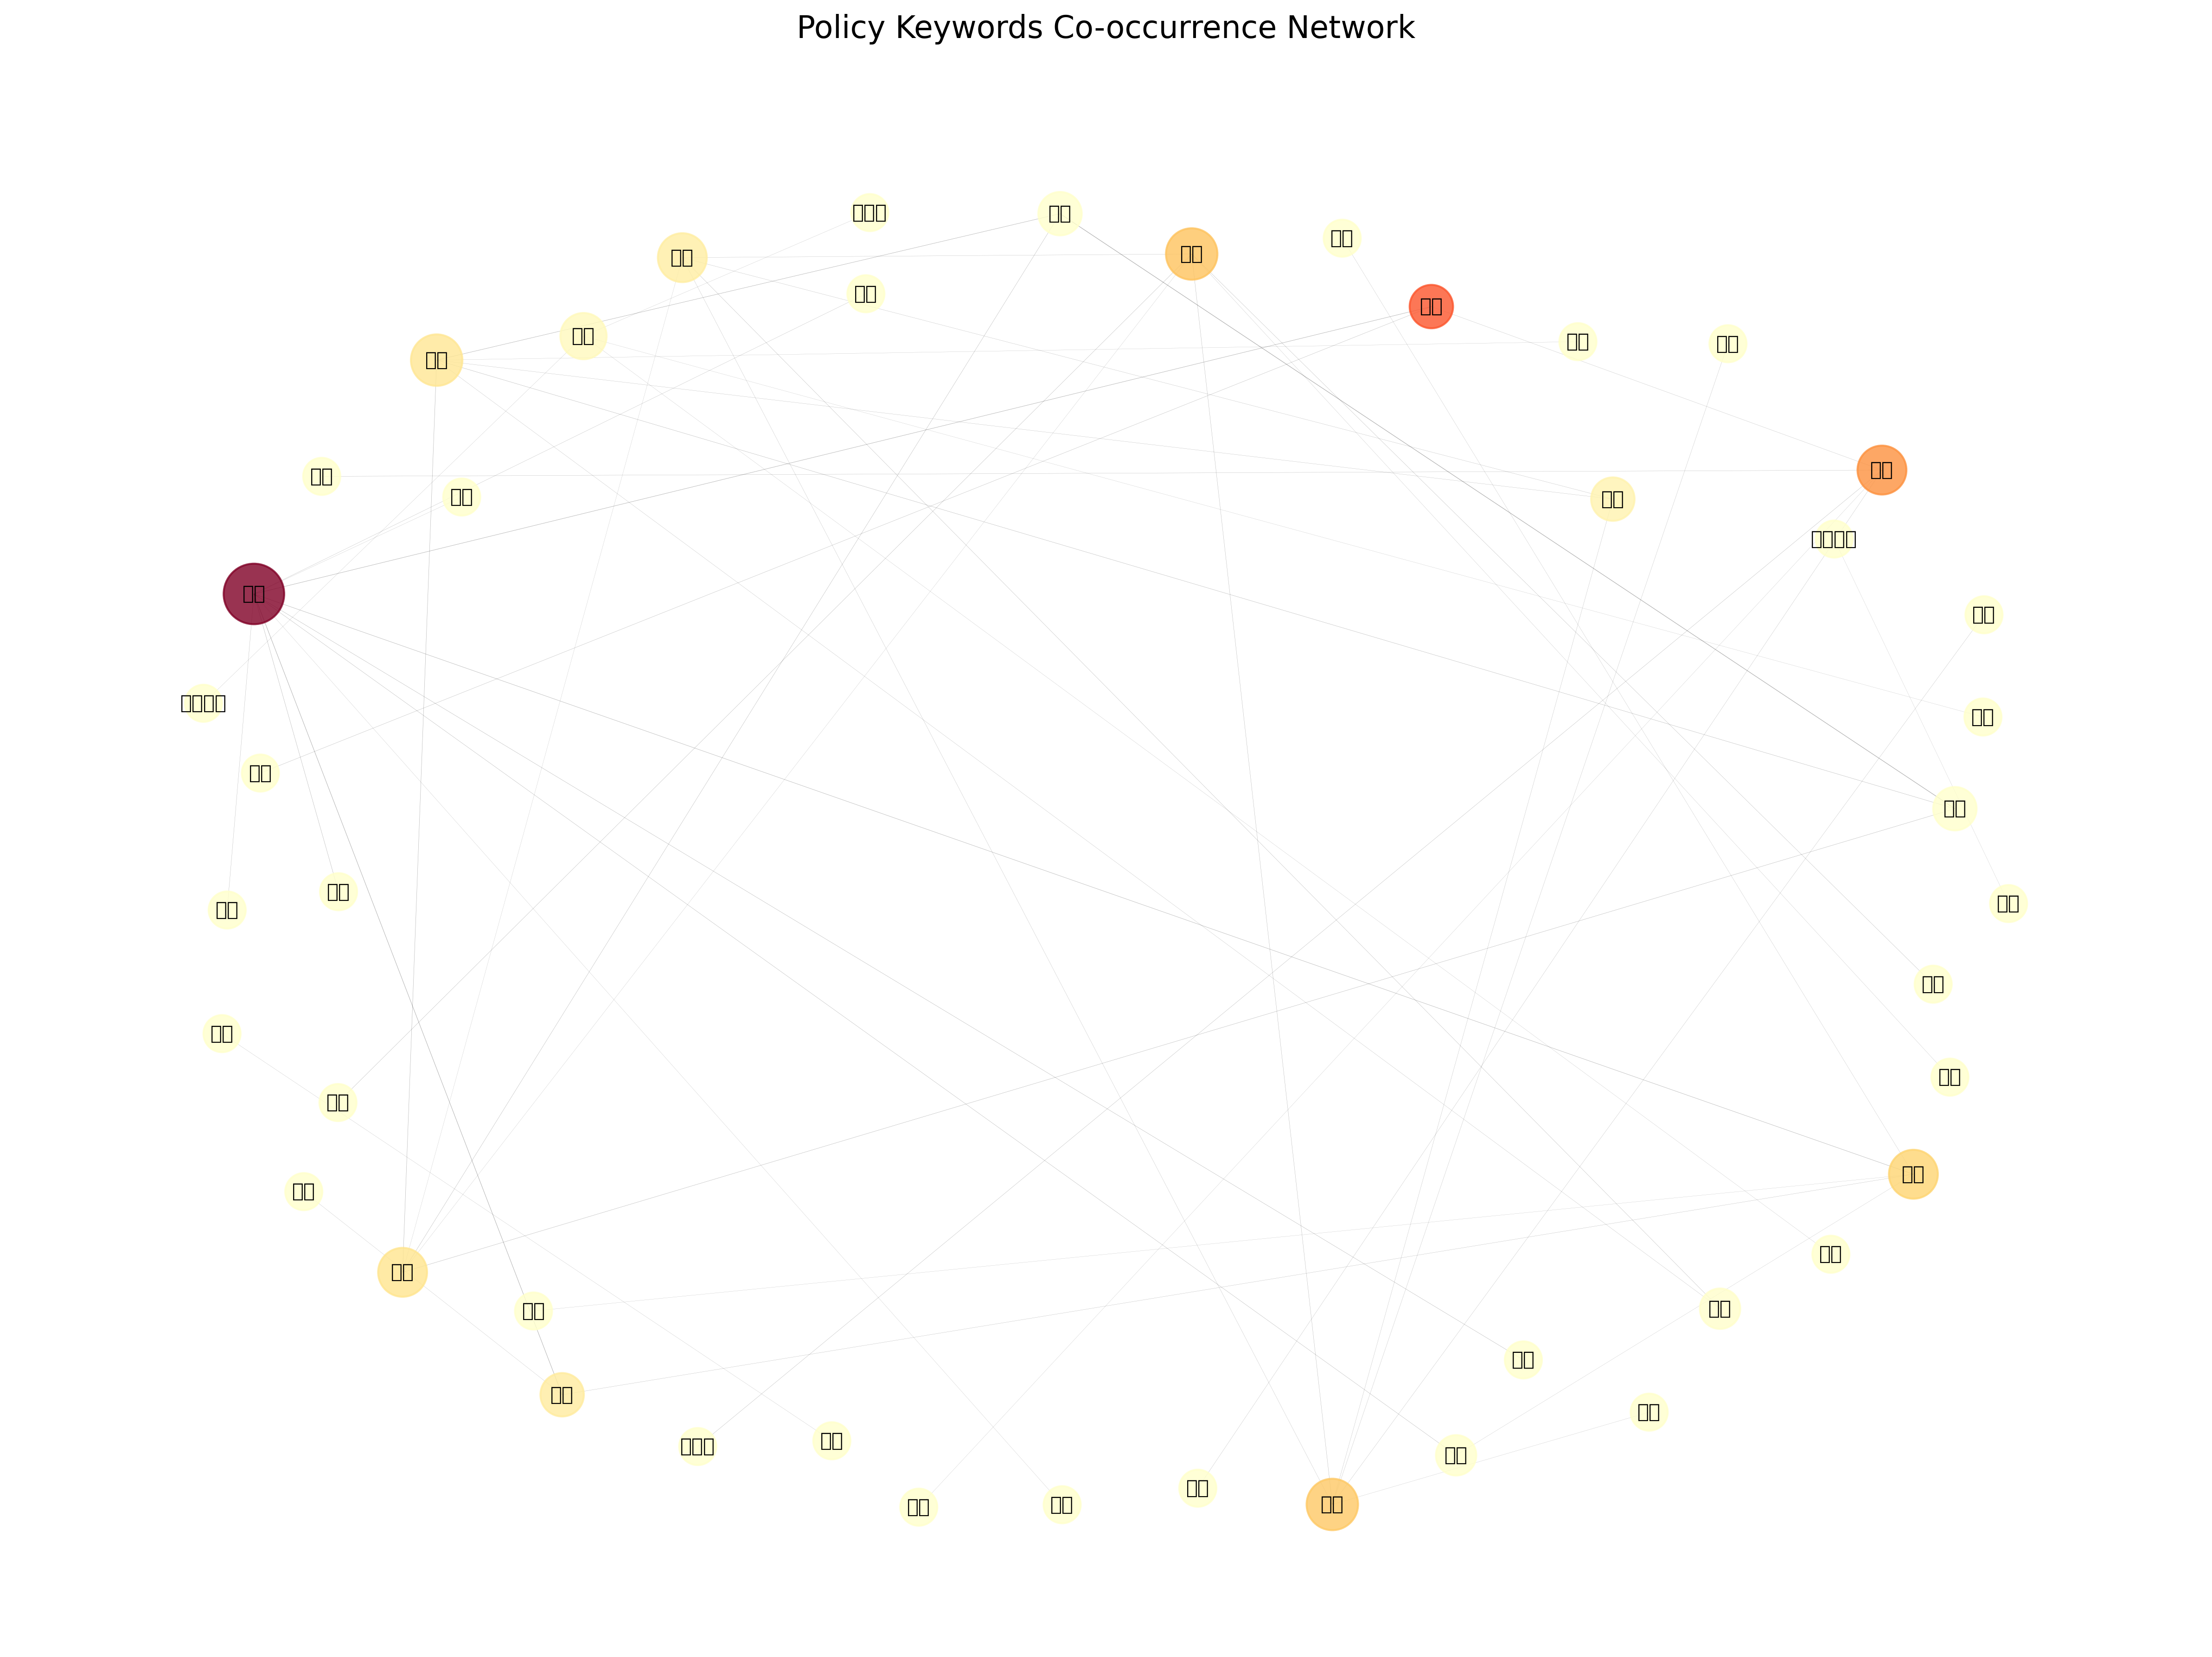
\includegraphics[width=0.95\textwidth]{figures/cooccurrence_network.png}
\caption{政策关键词共现网络图}
\label{fig:network}
\end{figure}

度中心性分析显示,"数据"(0.227)、"智能"(0.136)、"能力"(0.136)、"评价"(0.136)、"研究"(0.114)为网络中最核心的节点。介数中心性分析则发现"数据"、"伦理"、"教学"等词在网络中起到桥梁作用,连接不同的主题簇。

强共现关系TOP10包括:
\begin{enumerate}
\item 建设 $\leftrightarrow$ 平台 (0.148)
\item 伦理 $\leftrightarrow$ 数据 (0.117)
\item 保护 $\leftrightarrow$ 数据 (0.101)
\item 智能 $\leftrightarrow$ 建设 (0.093)
\item 研究 $\leftrightarrow$ 数据 (0.089)
\item 教学 $\leftrightarrow$ 智能 (0.079)
\item 防止 $\leftrightarrow$ 数据 (0.073)
\item 确保 $\leftrightarrow$ 数据 (0.072)
\item 教学 $\leftrightarrow$ 平台 (0.072)
\item 智能 $\leftrightarrow$ 平台 (0.071)
\end{enumerate}

可以发现,"数据"一词在多个共现对中出现,与"伦理"、"保护"、"研究"、"防止"、"确保"等词紧密相关,凸显了数据安全和隐私保护在政策中的核心地位。同时,"平台-建设"、"智能-教学"等共现关系反映了高校重视智能教学平台建设。

\subsection{关键词聚类}

使用K-means算法对关键词进行聚类,识别出5个语义簇(图\ref{fig:cluster}):

\begin{figure}[H]
\centering
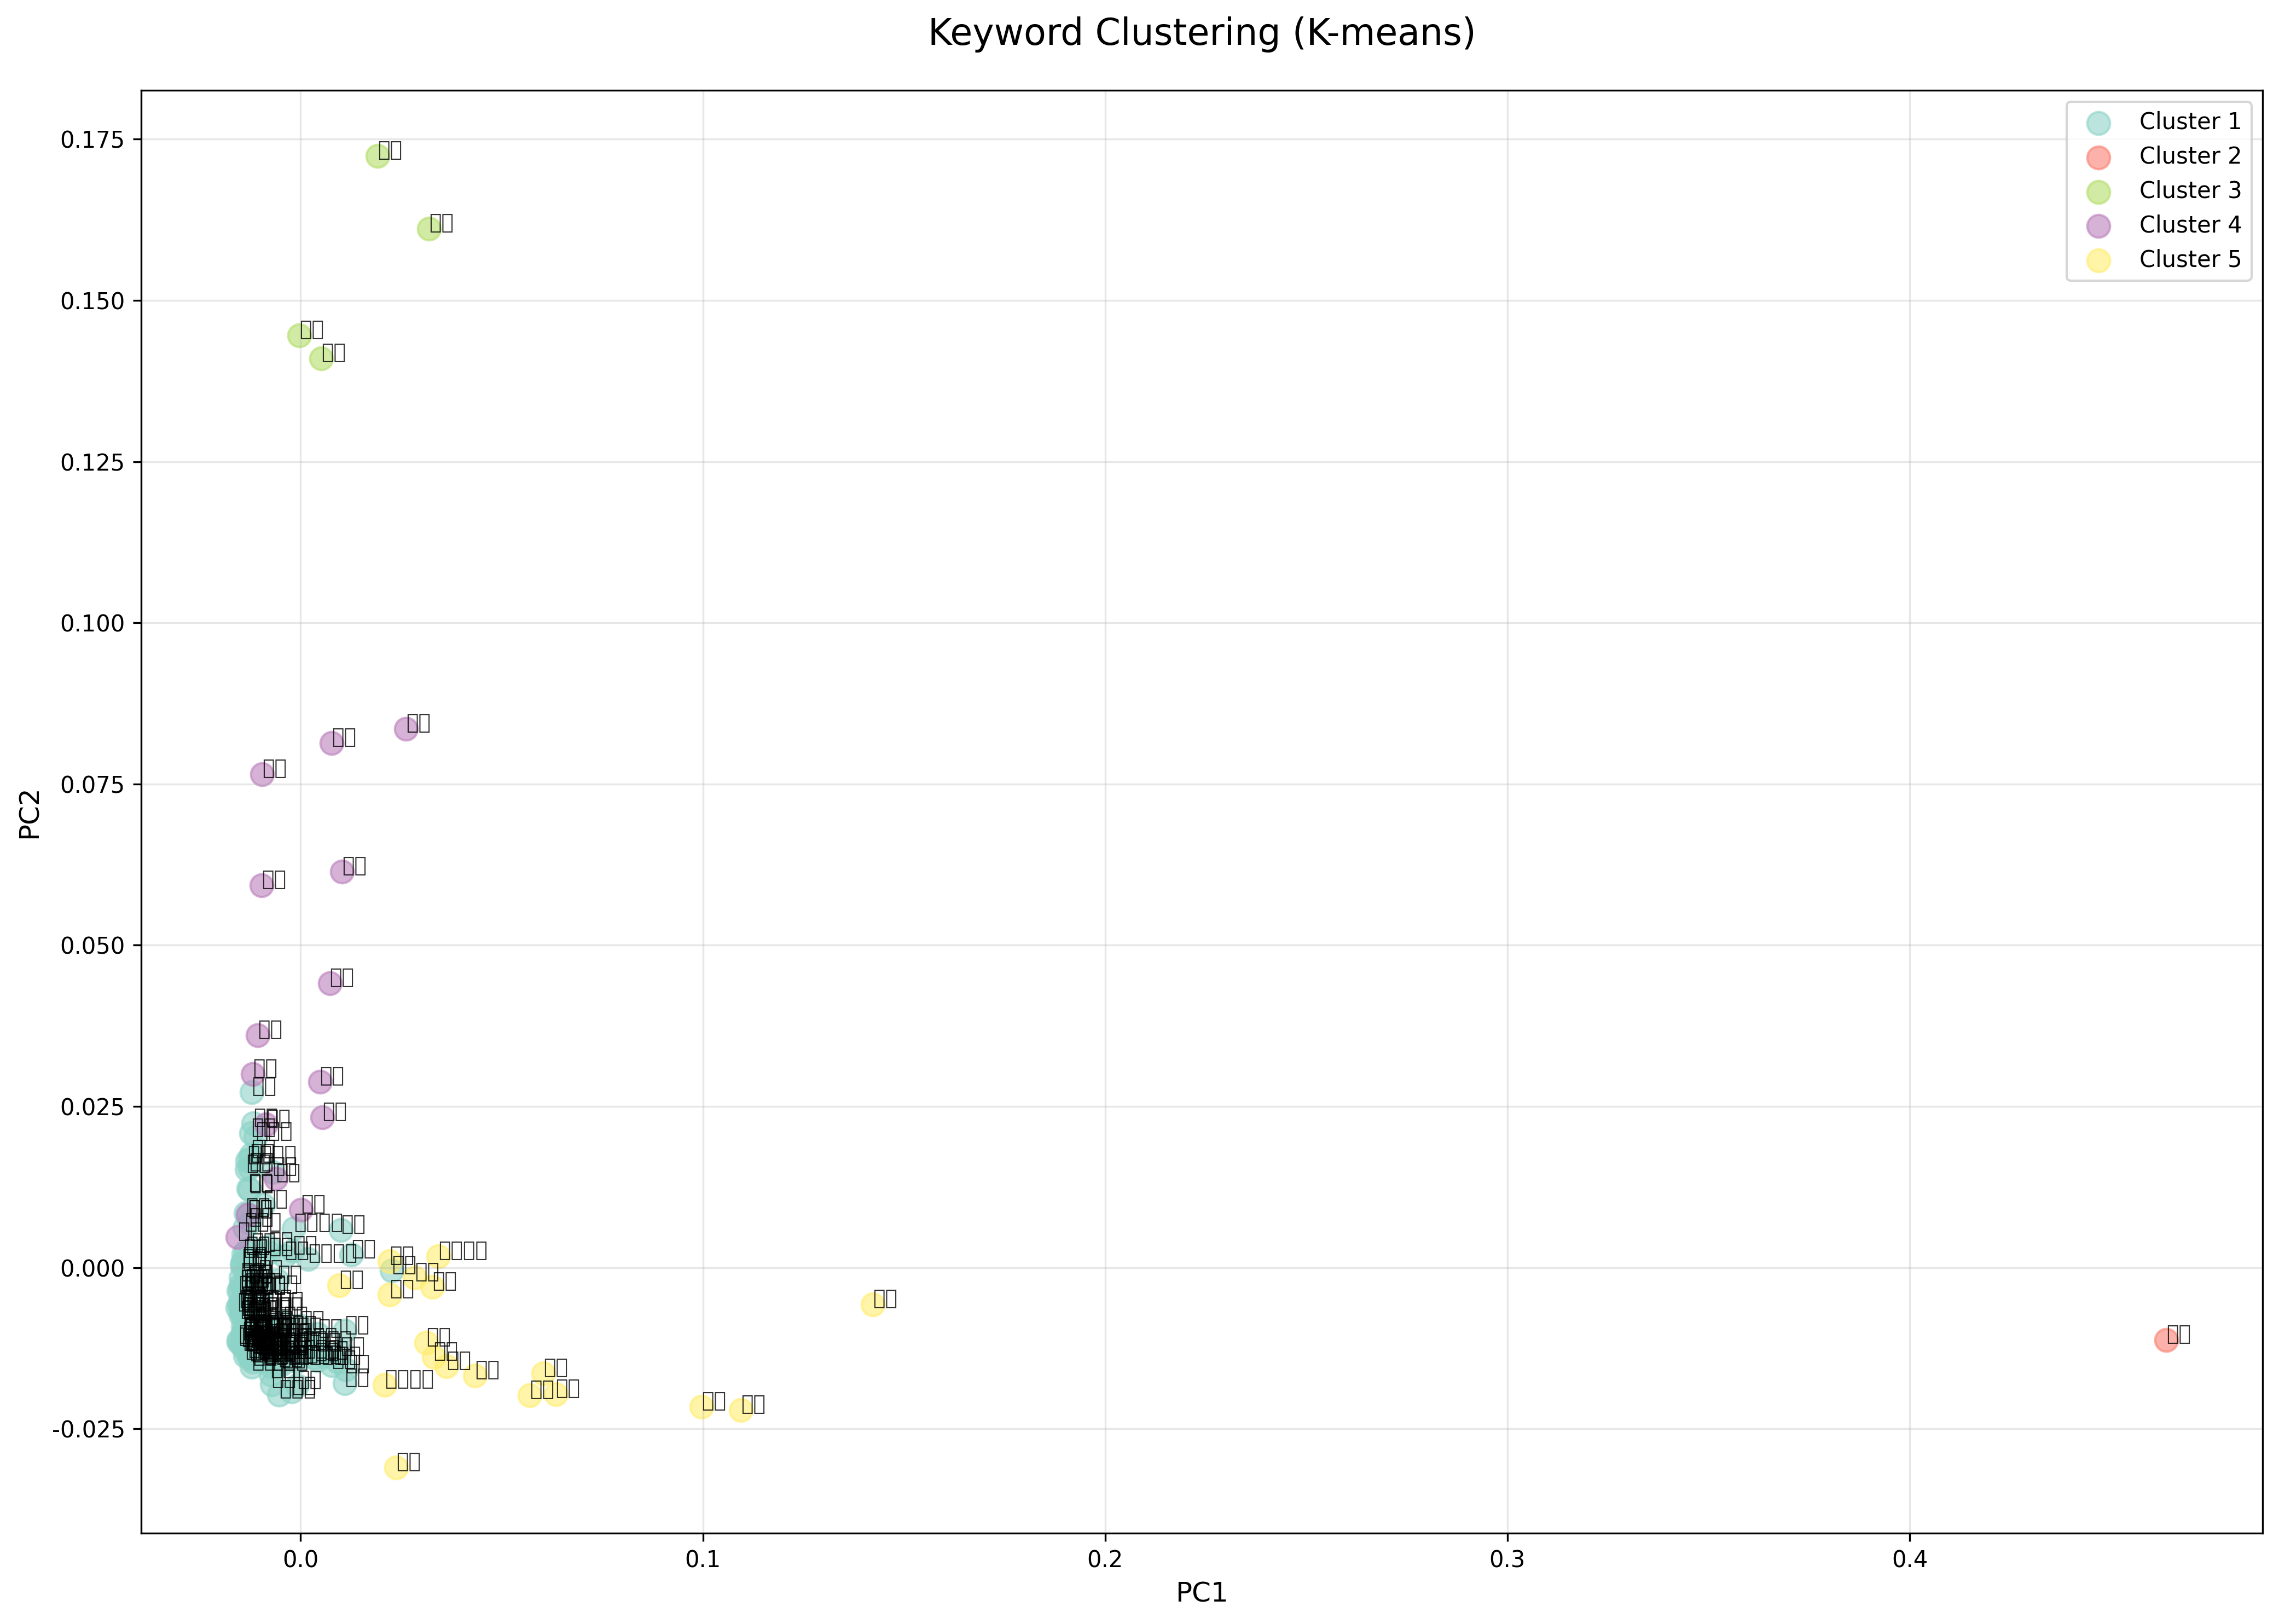
\includegraphics[width=0.85\textwidth]{figures/keyword_clusters.png}
\caption{关键词聚类分析}
\label{fig:cluster}
\end{figure}

\textbf{簇1:数据安全与隐私保护}——包含"数据"、"伦理"、"保护"、"隐私"、"防止"、"确保"等词,反映政策对数据安全的高度重视。

\textbf{簇2:教学应用与平台建设}——包含"教学"、"智能"、"平台"、"建设"、"资源库"、"研讨"等词,体现了AI赋能教学的政策导向。

\textbf{簇3:能力培养与创新}——包含"能力"、"培养"、"创新"、"学生"、"教师"、"素养"等词,强调师生AI素养提升。

\textbf{簇4:科研规范与管理}——包含"研究"、"科研"、"论文"、"项目"、"办法"、"规定"等词,关注AI在科研中的规范使用。

\textbf{簇5:评价改革与体系建设}——包含"评价"、"体系"、"改革"、"机制"、"质量"等词,反映教育评价变革诉求。

\subsection{不同类别政策的特征}

表\ref{tab:category}总结了不同类别政策的关键词特征:

\begin{table}[H]
\centering
\caption{不同类别政策的高频关键词}
\label{tab:category}
\small
\begin{tabular}{lp{10cm}}
\toprule
政策类别 & 高频关键词(TOP5) \\
\midrule
教学管理 & AI(19), 使用(12), 技术(9), 应用(7), 规范(6) \\
伦理规范 & AI(29), 使用(12), 伦理(11), 数据(9), 技术(6) \\
技术管理 & AI(9), 技术(7), 应用(7), 管理(3), 要求(3) \\
教学改革 & AI(13), 教学(6), 创新(5), 技术(4), 教育(4) \\
学生指导 & AI(14), 使用(11), 可能(4), 工具(4), 生成(3) \\
教师指导 & AI(16), 评价(6), 使用(6), 教学(5), 学生(5) \\
科研管理 & 使用(15), AI(14), 数据(8), 研究(5), 规定(4) \\
发展规划 & AI(21), 教学(7), 体系(5), 教育(4), 评价(4) \\
\bottomrule
\end{tabular}
\end{table}

从表中可以看出:
\begin{itemize}
\item 所有类别政策都将"AI"和"使用"作为核心关键词;
\item 伦理规范类政策突出"伦理"、"数据",体现价值导向;
\item 教学改革类强调"创新"、"教育",聚焦改革创新;
\item 科研管理类侧重"数据"、"研究"、"规定",注重规范约束;
\item 发展规划类关注"体系"、"评价",具有战略性和系统性。
\end{itemize}

\subsection{主题演化分析}

按时间顺序分析政策主题,发现明显的演化趋势(图\ref{fig:evolution}):

\begin{figure}[H]
\centering
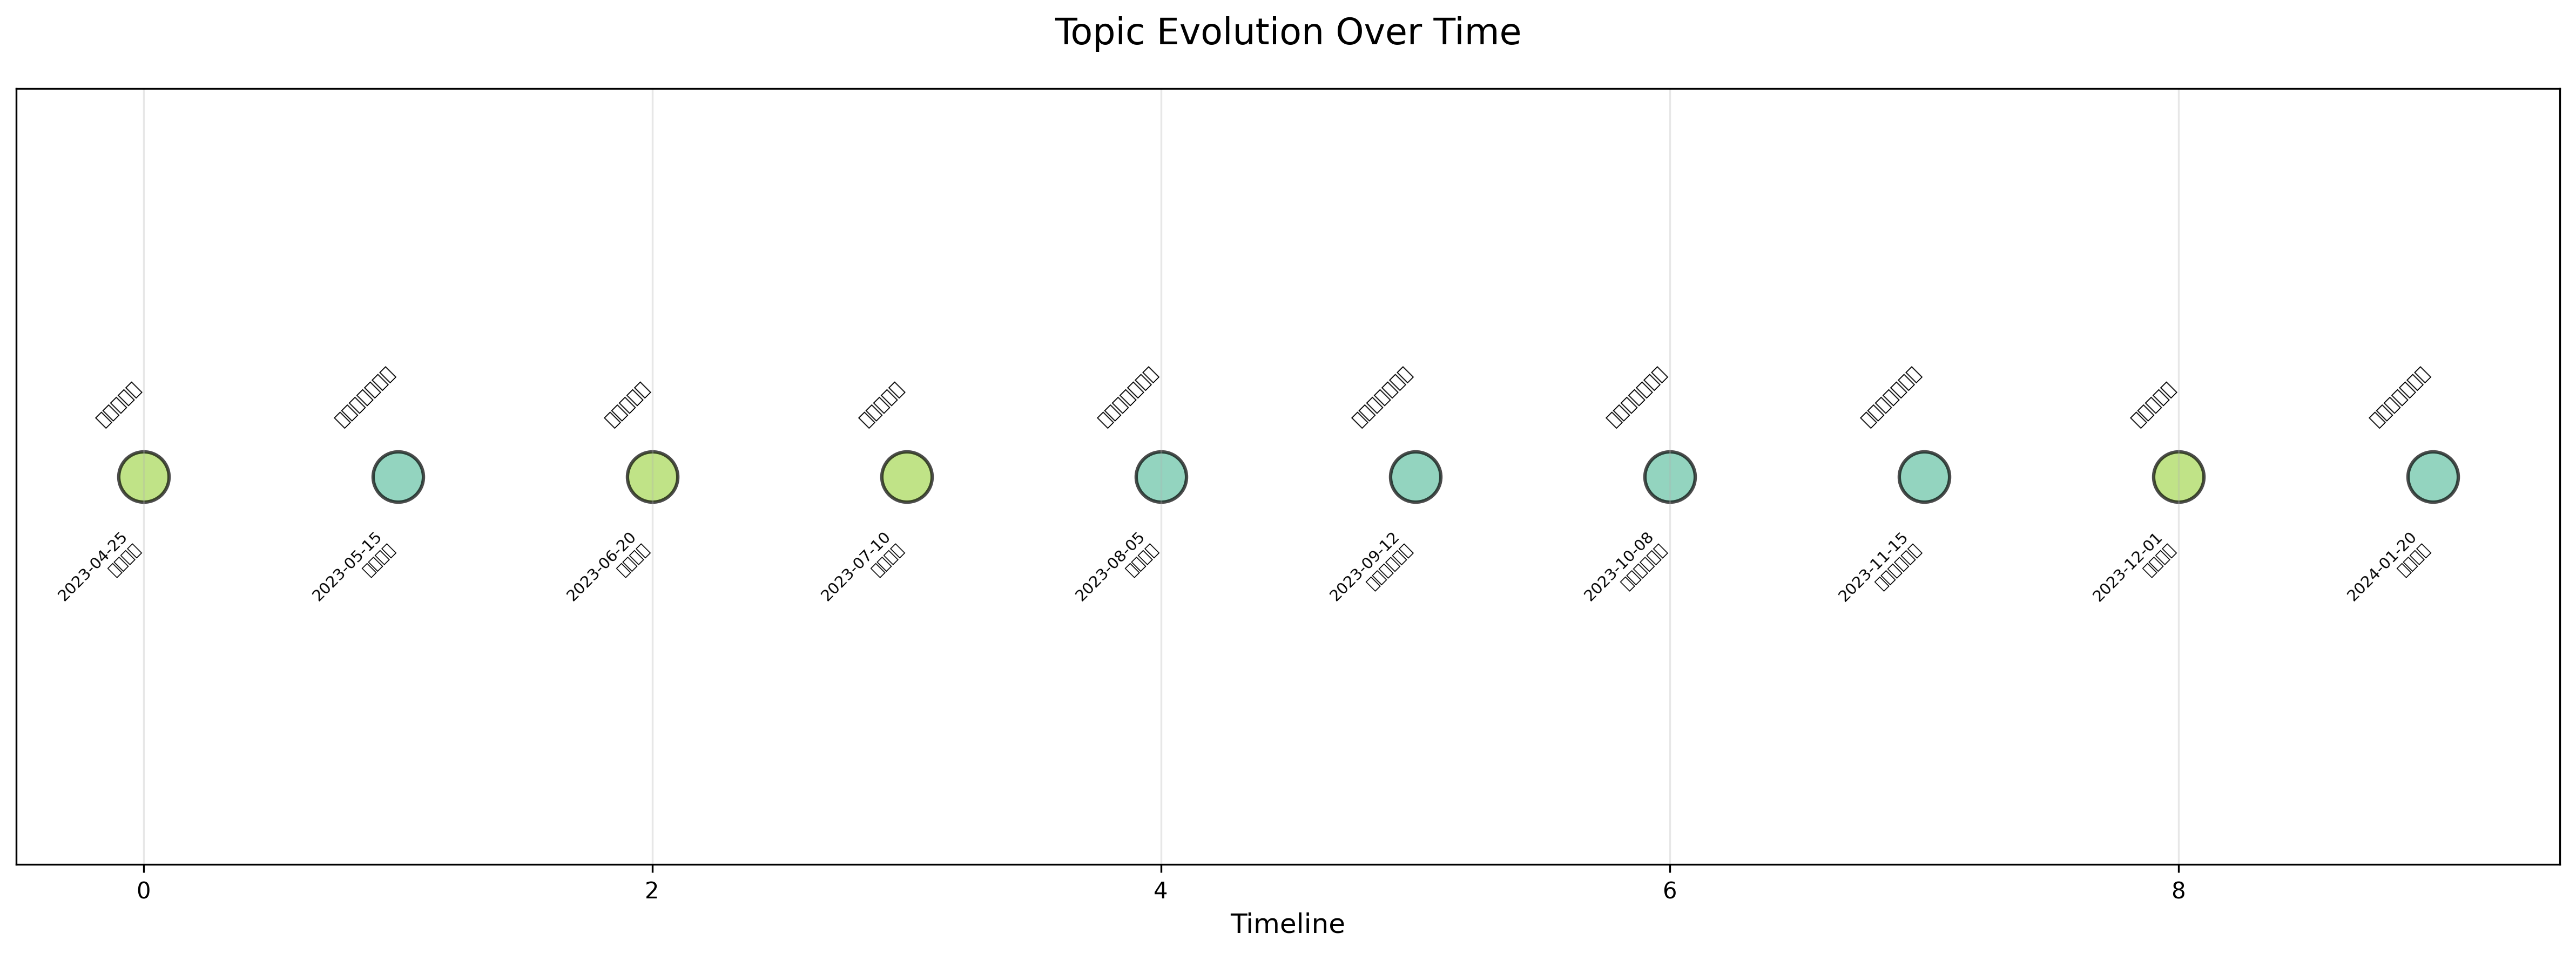
\includegraphics[width=0.95\textwidth]{figures/topic_evolution.png}
\caption{政策主题演化时间线}
\label{fig:evolution}
\end{figure}

\textbf{阶段一(2023年4月-7月):伦理规范先行}——这一时期发布的政策多关注"伦理与规范"主题,如南京大学、北京大学、复旦大学的政策均侧重于建立AI使用的伦理准则和规范框架。这反映了高校在技术初期的审慎态度。

\textbf{阶段二(2023年8月-2024年1月):转向应用创新}——随着对技术的认识深化,政策主题逐渐转向"教学应用与创新",如浙江大学、上海交通大学、中国人民大学、北京师范大学、中山大学的政策更多关注AI如何赋能教学改革和创新。

这一演化趋势与穆卫军等\cite{ref10}发现的教育政策从"规范"到"提质"的转变相一致,也印证了易璐等\cite{ref3}关于政策关注点从上游向下游、从防范向应用转移的规律。

\section{讨论}

\subsection{政策特征总结}

本研究发现,国内双一流高校生成式AI政策呈现以下特征:

\textbf{(1) 价值导向明确:}政策始终坚持"育人为本"原则,强调技术服务于人的全面发展,反对技术异化。这与颜志萍等\cite{ref1}揭示的公众对AI安全的价值关切一致。

\textbf{(2) 风险意识突出:}数据安全、隐私保护、学术诚信在政策中占据重要位置,反映了高校对AI技术双刃剑特性的清醒认识。

\textbf{(3) 应用导向渐强:}从早期的规范约束转向鼓励创新应用,体现了政策的动态调适特征。这与刘滢等\cite{ref7}发现的叙事框架从抽象转向具体实践的趋势相符。

\textbf{(4) 多元主体关照:}政策涵盖教师、学生、管理人员等多个群体,体现了协同治理理念,与许世建等\cite{ref4}强调的多主体参与相呼应。

\subsection{政策启示}

基于研究发现,提出以下政策建议:

\textbf{(1) 加强顶层设计:}建议高校制定系统性的AI应用发展规划,统筹教学、科研、管理等各领域政策,避免碎片化。

\textbf{(2) 完善保障机制:}在重视规范的基础上,需加大对AI教育教学应用的资源投入,建设安全可靠的校级AI服务平台。

\textbf{(3) 强化能力建设:}将AI素养教育纳入师生培训体系,提升全员的技术应用能力和伦理意识,这与俞立平等\cite{ref8}强调的人才培养工具重要性一致。

\textbf{(4) 推动评价改革:}适应AI时代要求,创新考核评价方式,减少死记硬背,增加批判性思维和创新能力考查。

\textbf{(5) 促进交流共享:}建立高校间AI政策和最佳实践分享机制,推动形成共识,避免重复探索。

\subsection{研究局限}

本研究存在以下局限:

\textbf{(1) 样本规模有限:}仅收集了10所高校的政策文本,未来可扩大样本范围,涵盖更多高校和政策类型。

\textbf{(2) 时间跨度较短:}数据覆盖不足一年,难以捕捉长期演化趋势。随着政策的持续更新,需要开展追踪研究。

\textbf{(3) 方法局限:}文本分析主要揭示"说什么",难以评估政策的实际执行效果和影响,需要结合访谈、问卷等方法深入研究。

\section{结论}

本研究综合运用TF-IDF、LDA主题模型和语义网络分析方法,对国内10所双一流高校的生成式人工智能政策进行了系统分析。研究发现,高校政策在保持价值导向和风险意识的同时,呈现出从规范约束向创新应用转变的趋势。数据安全、学术诚信、教学创新、能力培养构成政策核心议题。不同类别政策各有侧重,但均强调AI技术的负责任使用。

研究为理解国内高校生成式AI政策的特征和演化提供了实证依据,对高校完善相关政策、推动AI与教育深度融合具有参考价值。未来研究可以扩大样本范围,延长观察时间,结合多种研究方法,深入探讨政策的实施效果和影响机制。

\begin{thebibliography}{99}

\bibitem{ref1} 颜志萍. 人工智能安全的公众认知研究——基于在线评论的文本分析[J]. 情报杂志, 2023.

\bibitem{ref2} 魏澜. 我国职业教育学生实习政策演变研究——基于68份政策文本的加权共词分析[J]. 职业技术教育, 2023.

\bibitem{ref3} 易璐. 中国稀土产业政策演进研究(1991—2021)——基于共词和社会语义网络分析[J]. 中国矿业, 2022.

\bibitem{ref4} 许世建. 企业参与职业教育办学的政府注意力演化——基于1978—2021年国家产教融合政策的文本分析[J]. 教育发展研究, 2023.

\bibitem{ref5} 陈翔. 基于动态语义网络分析的主题演化路径识别研究[J]. 情报学报, 2022.

\bibitem{ref6} 巴志超. 基于关键词语义网络的领域主题演化分析方法研究[J]. 图书情报工作, 2022.

\bibitem{ref7} 刘滢. "人类命运共同体"理念的国际社交媒体呈现——基于Twitter平台的内容分析和语义网络分析[J]. 新闻与传播研究, 2023.

\bibitem{ref8} 俞立平. 政策工具视角下科技创新质量相关政策演化特征研究——基于2000–2022年政策文本分析[J]. 科技进步与对策, 2023.

\bibitem{ref9} 楚东晓. 基于LDA和语义网络的产品感知价值维度研究[J]. 管理评论, 2022.

\bibitem{ref10} 穆卫军. 新时代我国高等学历继续教育政策文本的语义网络分析[J]. 继续教育研究, 2023.

\end{thebibliography}

\appendix

\section{附录:可视化图表}

\begin{figure}[H]
\centering
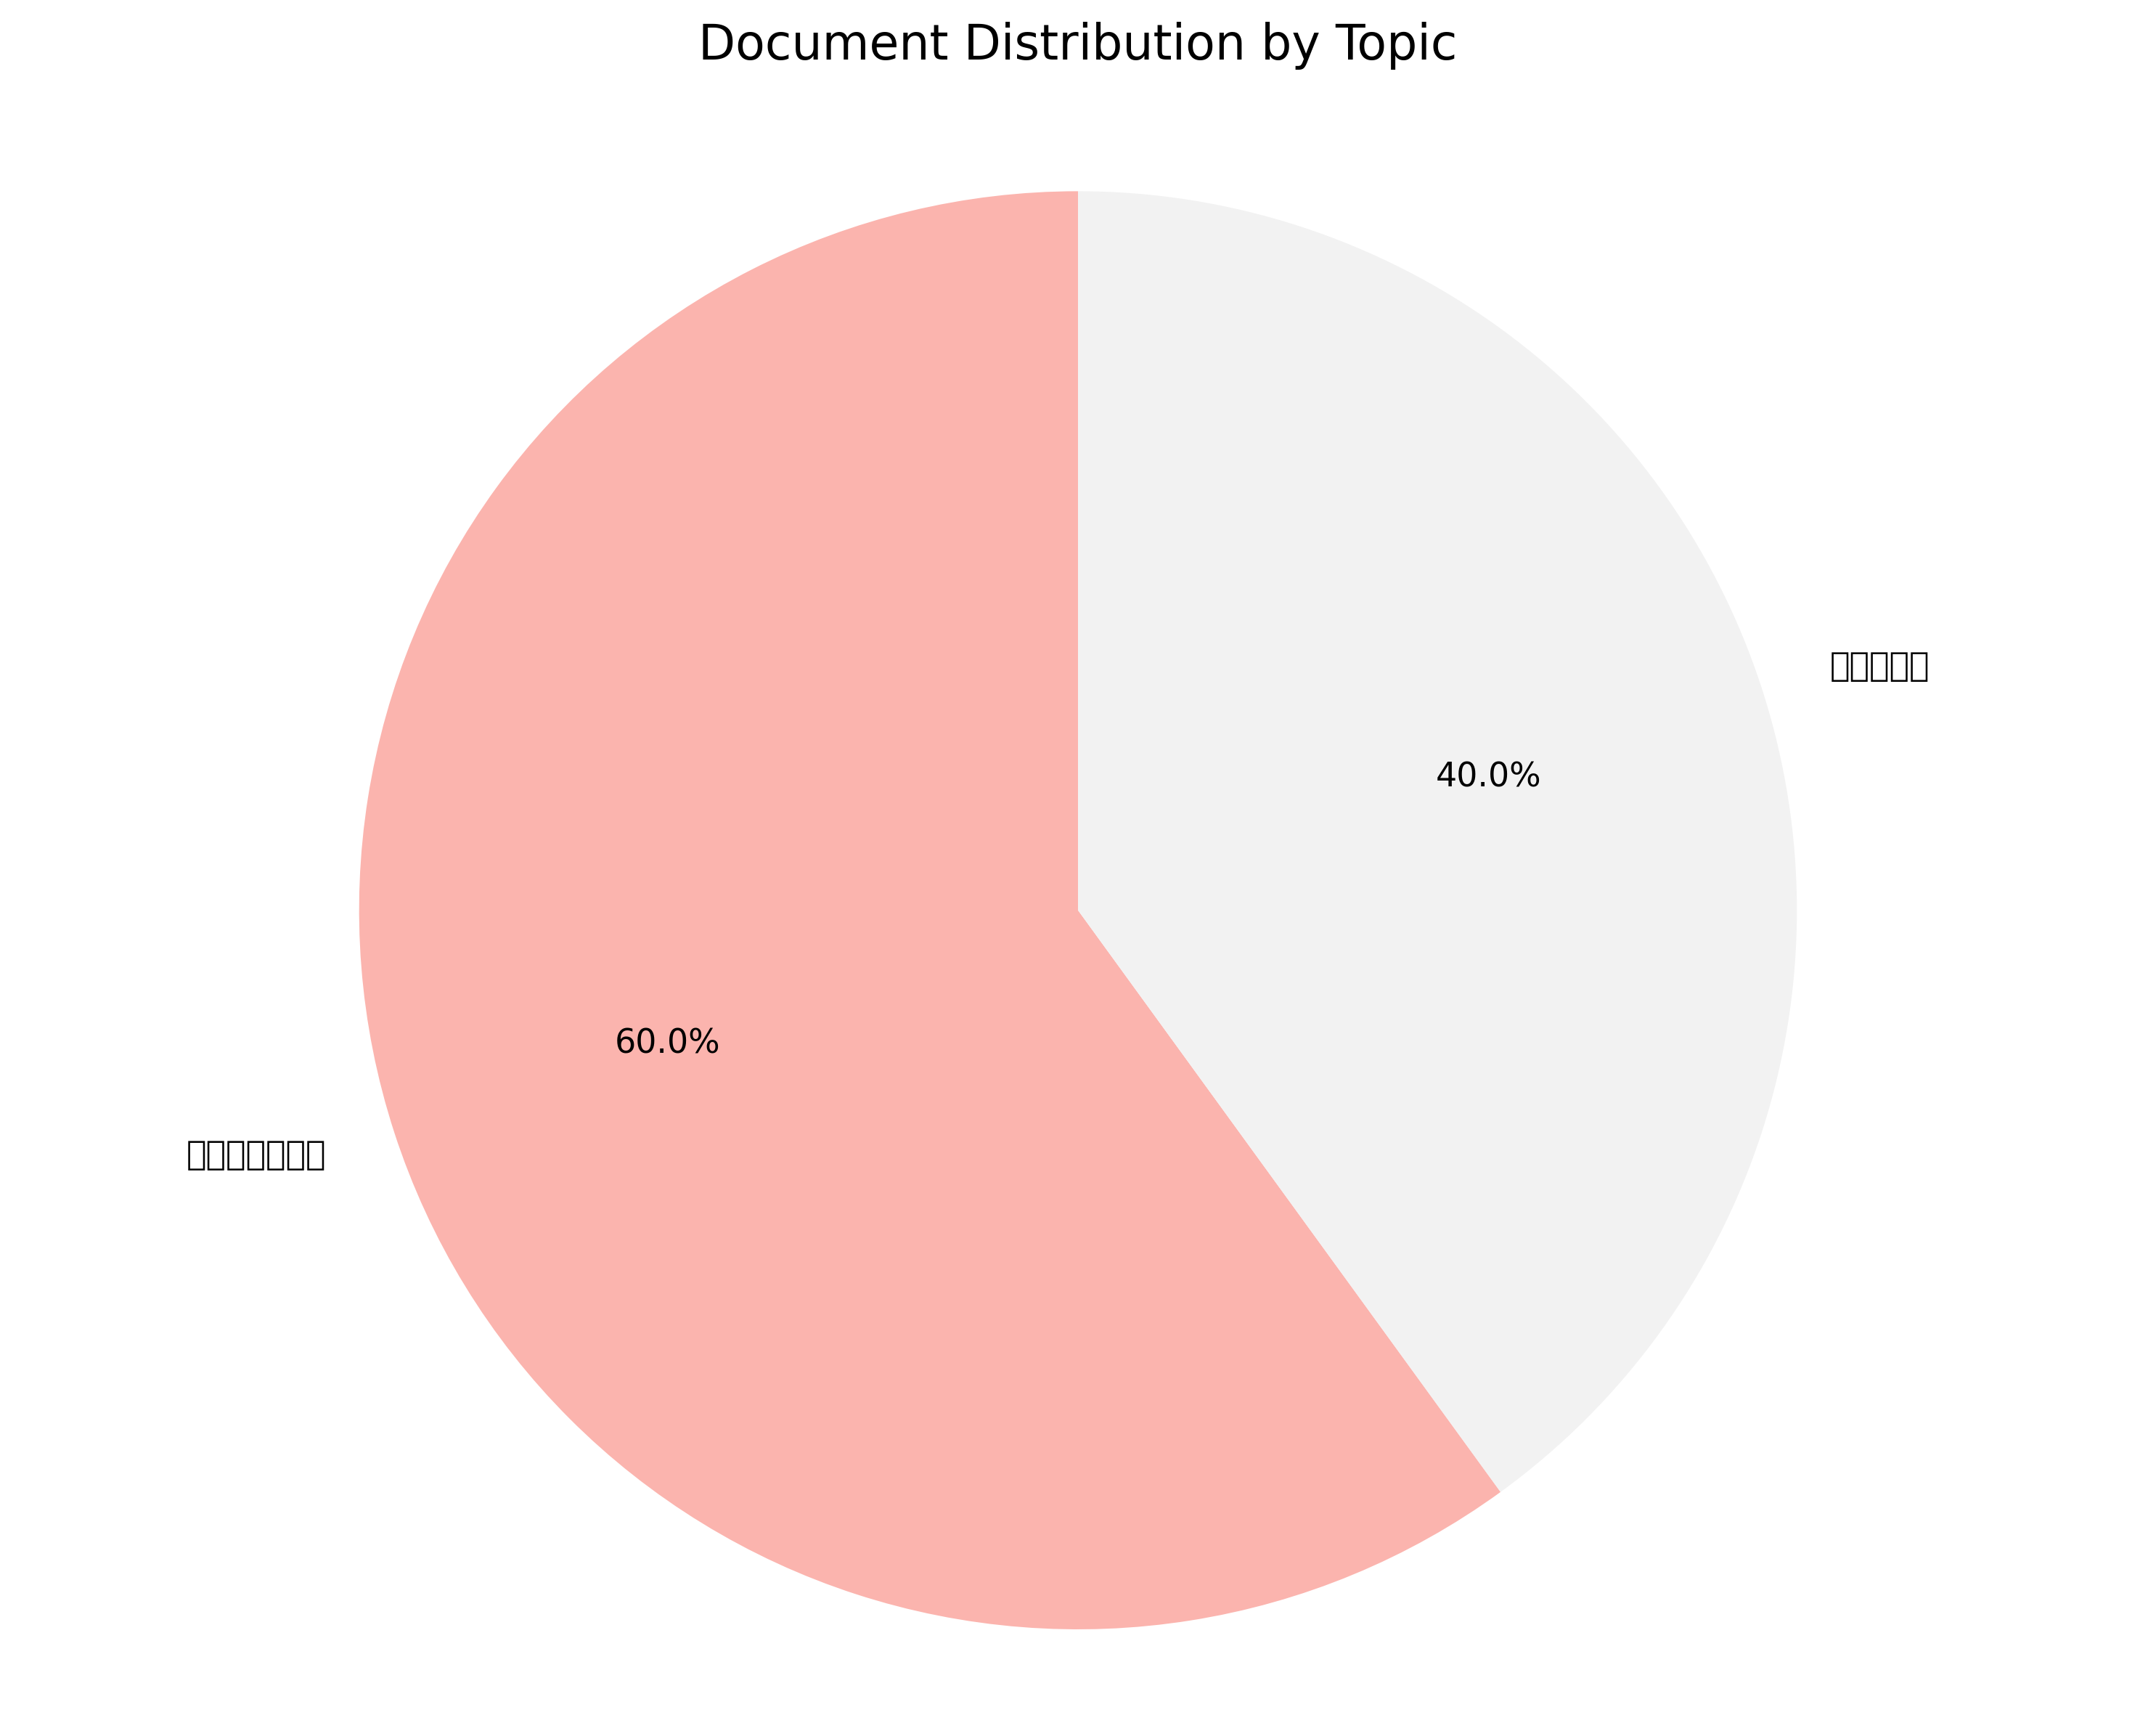
\includegraphics[width=0.8\textwidth]{figures/topic_distribution.png}
\caption{文档主题分布饼图}
\end{figure}

\begin{figure}[H]
\centering
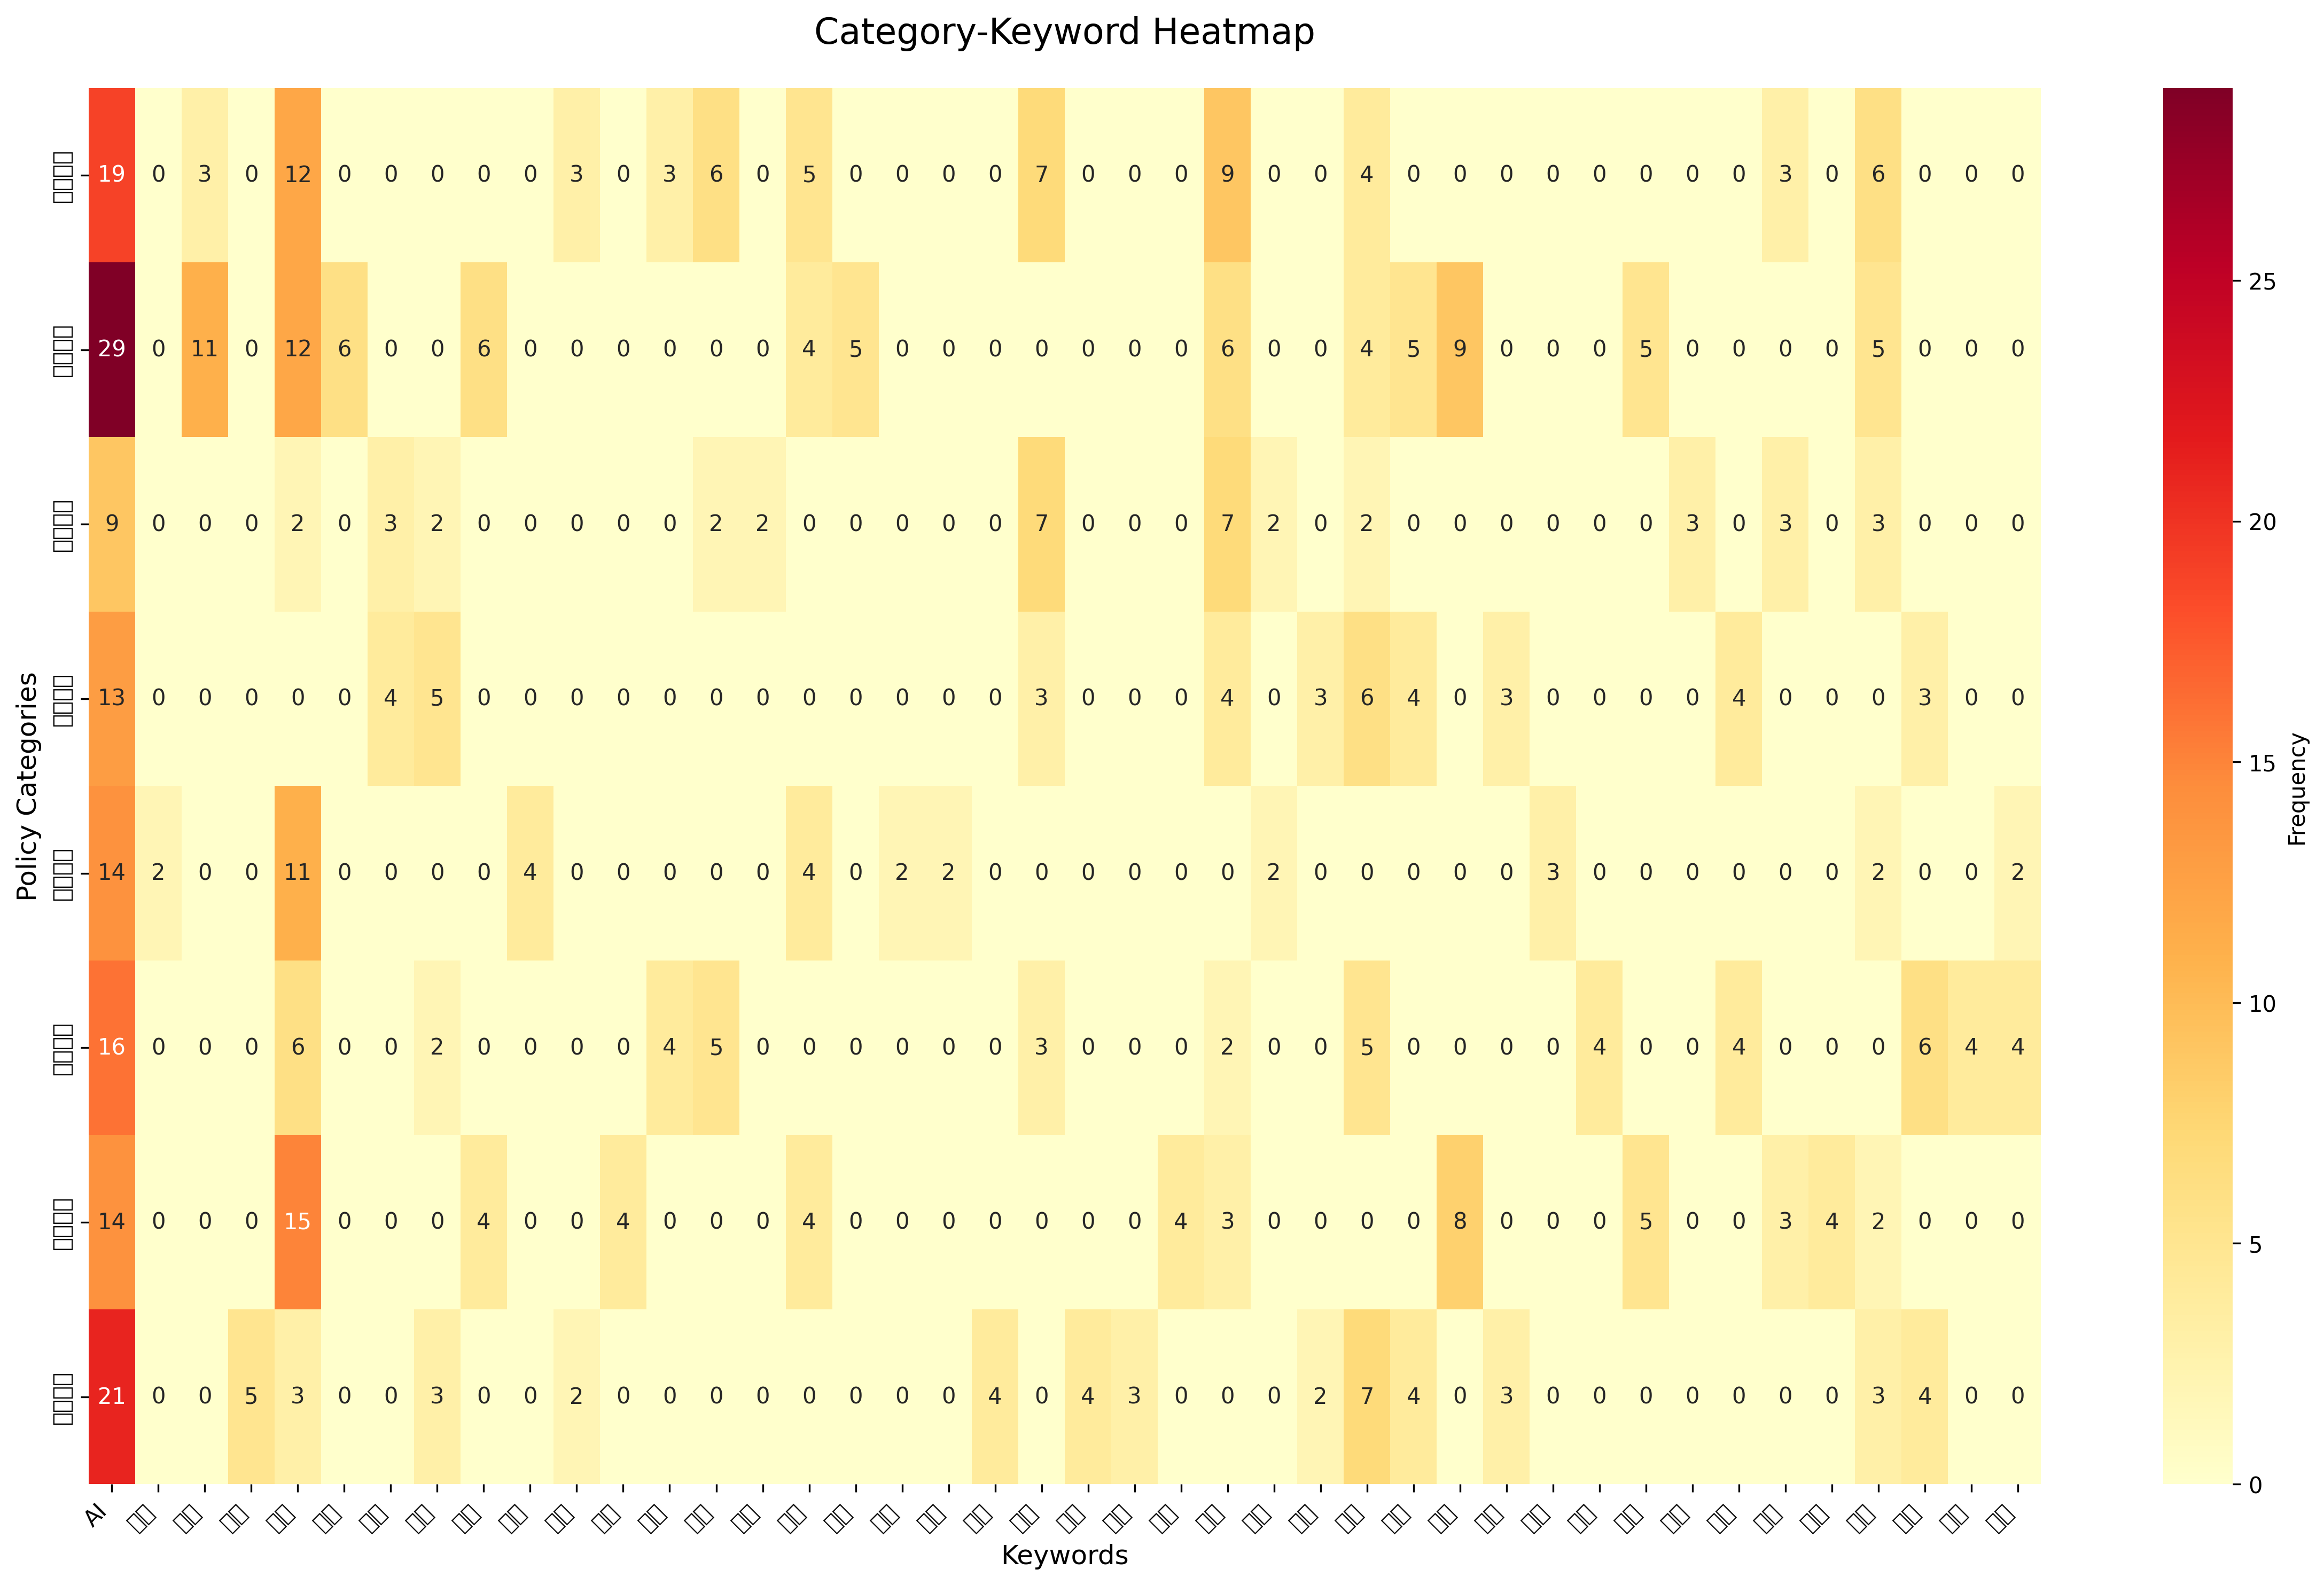
\includegraphics[width=0.9\textwidth]{figures/category_keywords_heatmap.png}
\caption{政策类别-关键词热力图}
\end{figure}

\begin{figure}[H]
\centering
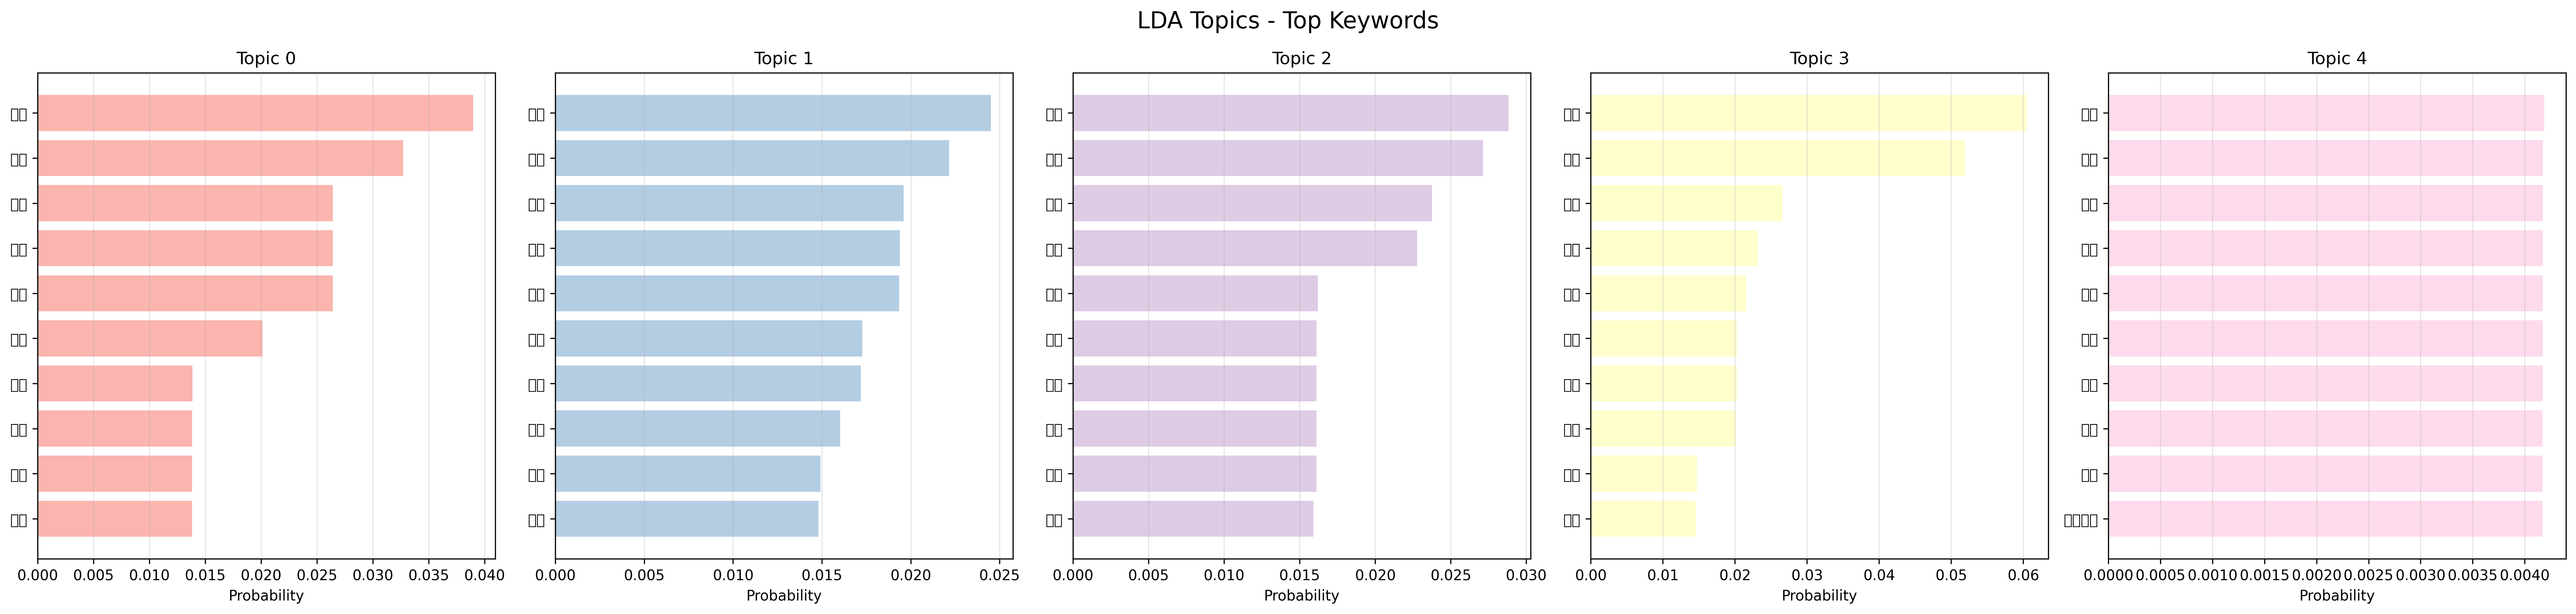
\includegraphics[width=0.9\textwidth]{figures/lda_topics_bar.png}
\caption{LDA主题关键词分布}
\end{figure}

\end{document}
